%!TEX root = ../dissertation.tex
\chapter{Code}
\label{AppendixA}
The following code are the major functions written to perform the investigation here were written in Python 3.  The functions follow the protocol lain out in Chapter \ref{Methods}.  


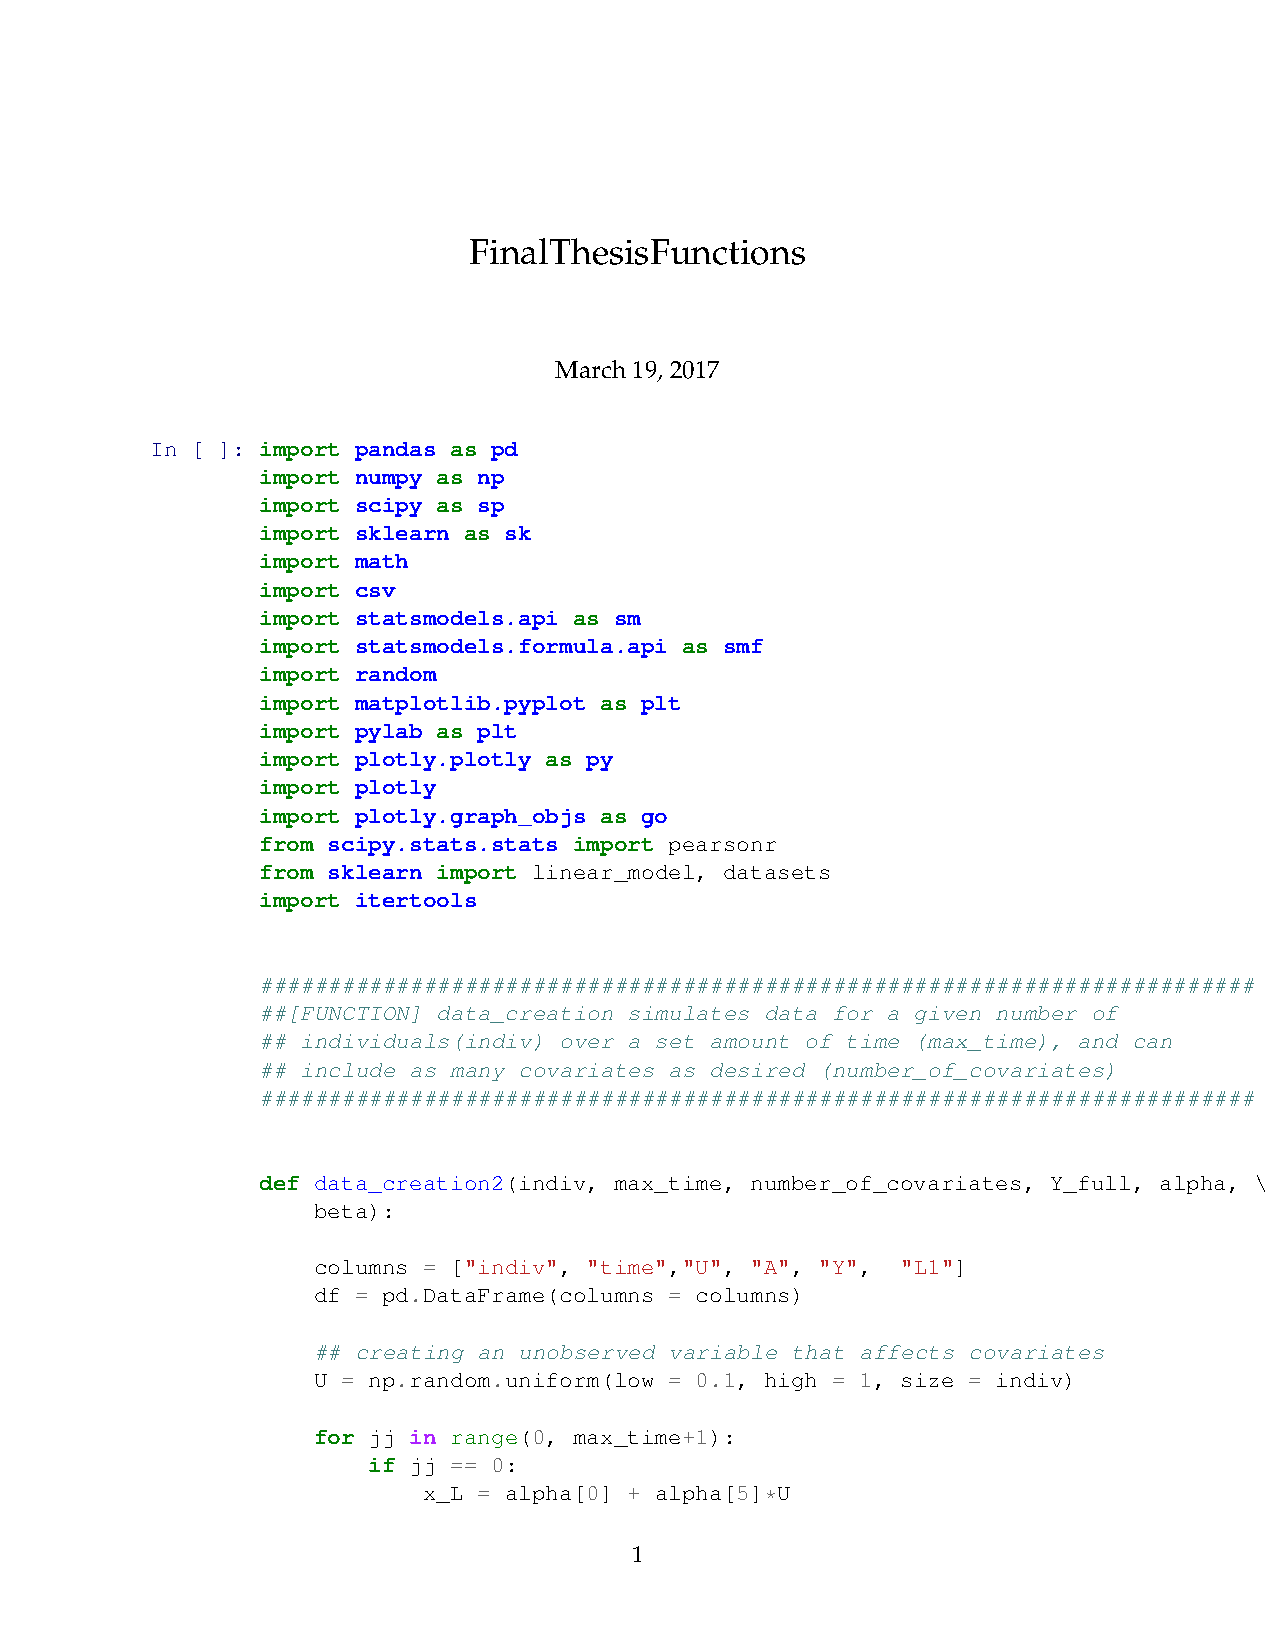
\includepdf[
    pages=-,
    %% make this page have the usual page style
    %% (you can change it to plain etc). By default pdfpages
    %% sets the pagecommand to \pagestyle{empty}
    pagecommand={\pagestyle{headings}}, 
    offset=0 25, 
    width = 155mm, 
    height = 220mm, 
    %% Add a "section" entry to the ToC with the heading
    %% "Quilling Shapes" and the label "sec:shapes"
    addtotoc={1,section,1,Python Functions,sec:shapes}]
    {../FinalThesisFunctions.pdf}
    
\chapter{Extra Math} \label{AppendixB}

\begin{table}[h!]
\centering
\begin{tabular} {c | c  c}
Model Correctly Specified & \shortstack{Average Bias \\ of Estimate}  & \shortstack{Std. Error \\of Bias} \\ 
\hline  \\
$\pi_3, \dots, \pi_K$ & 0.026 & 0.005   \\ 
$\pi_3, \dots, \pi_{K-1}, s_K$ & 0.024 & 0.004\\ 
$\pi_3, \dots, \pi_{K-2}, s_{K-1}, s_K$ & 0.023 & 0.004\\ 
$\pi_3, \dots, \pi_{K-3}, s_{K-2} , s_{K-1}, s_K$ & 0.023  &0.004 \\ 
$\pi_3, \dots, \pi_{K-4}, s_{K-3}, \dots s_K $ & 0.023&0.004 \\ 
$\pi_3, \dots, \pi_{K-5}, s_{K-4}, \dots s_K $ &  0.023 &0.004\\ 
$\pi_3, \dots, \pi_{K-6}, s_{K-5}, \dots s_K $ &  0.023 & 0.004 \\ 
$\pi_3, \dots, \pi_{K-7}, s_{K-6}, \dots s_K $ &  0.024 & 0.004\\ 
$\pi_3, s_{4}, \dots s_K $ &  0.025& 0.004 \\ 
$s_3, \dots s_K$ & 0.026 & 0.044 \\ 
$s_3, \dots s_{10}, \pi_K$ & 0.027 & 0.025 \\
$s_3, \dots s_9, \pi_{10}, \pi_K$ &  0.028 & 0.017 \\ 
$s_3, \dots s_8, \pi_9, \dots \pi_K$ & 0.048 &0.026   \\ 
$s_3, \dots s_7, \pi_8, \dots \pi_K$ &  0.060 &  0.025   \\ 
$s_3, \dots s_6, \pi_7, \dots \pi_K$ & 0.064 &0.021 \\ 
$s_3, s_4, s_5, \pi_6, \dots \pi_K$ & 0.052 & 0.005  \\ 
$s_3, s_4, \pi_5, \dots \pi_K$ & 0.080 & 0.005 \\ 
$s_3, \pi_4, \dots \pi_K$ &  0.196 & 0.005 \\ 
$s_3, \pi_4, s_5, \pi_6, s_7, \pi_8, s_9, \pi_{10}, s_{11}$ & 0.031& 0.005 \\ 
$\pi_3, s_4, \pi_5, s_6, \pi_7, s_8, \pi_9, s_{10}, \pi_{11}$ & 0.034 & 0.005
\end{tabular} \\
\centering
\caption[Testing multiple robustness]{Further results of the testing of multiple robustness of the doubly robust method as described in Section \ref{multiplerobust}.}
\label{MultipleTable}
\end{table}
